\documentclass[12pt, twoside]{article}
\usepackage[francais]{babel}
\usepackage[T1]{fontenc}
\usepackage[latin1]{inputenc}
\usepackage[left=7mm, right=7mm, top=5mm, bottom=5mm]{geometry}
\usepackage{float}
\usepackage{graphicx}
\usepackage{array}
\usepackage{multirow}
\usepackage{amsmath,amssymb,mathrsfs} 
\usepackage{soul}
\usepackage{textcomp}
\usepackage{eurosym}
\usepackage{lscape}
 \usepackage{variations}
\usepackage{tabvar}
 
\pagestyle{empty}


\date{}

\begin{document}

\begin{center}
\LARGE{\ul{\textbf{Divisibilit�}}}

\end{center}


\bigskip



\section{Division euclidienne}

\ul{D�finiton}: Effectuer la \textbf{division euclidienne} d'un nombre entier,
appel� le \textbf{dividende}, par un nombre entier diff�rent de 0, appel� le
\textbf{diviseur}, revient  �trouver deux nombres entiers appel�s
\textbf{quotient} et le \textbf{reste}, v�rifiant:


\begin{center}
\textbf{dividende}= \textbf{diviseur} $\times$ \textbf{quotient} +
\textbf{reste} avec reste < diviseur
\end{center}



\enskip


\ul{Exemple}: 

\begin{center}
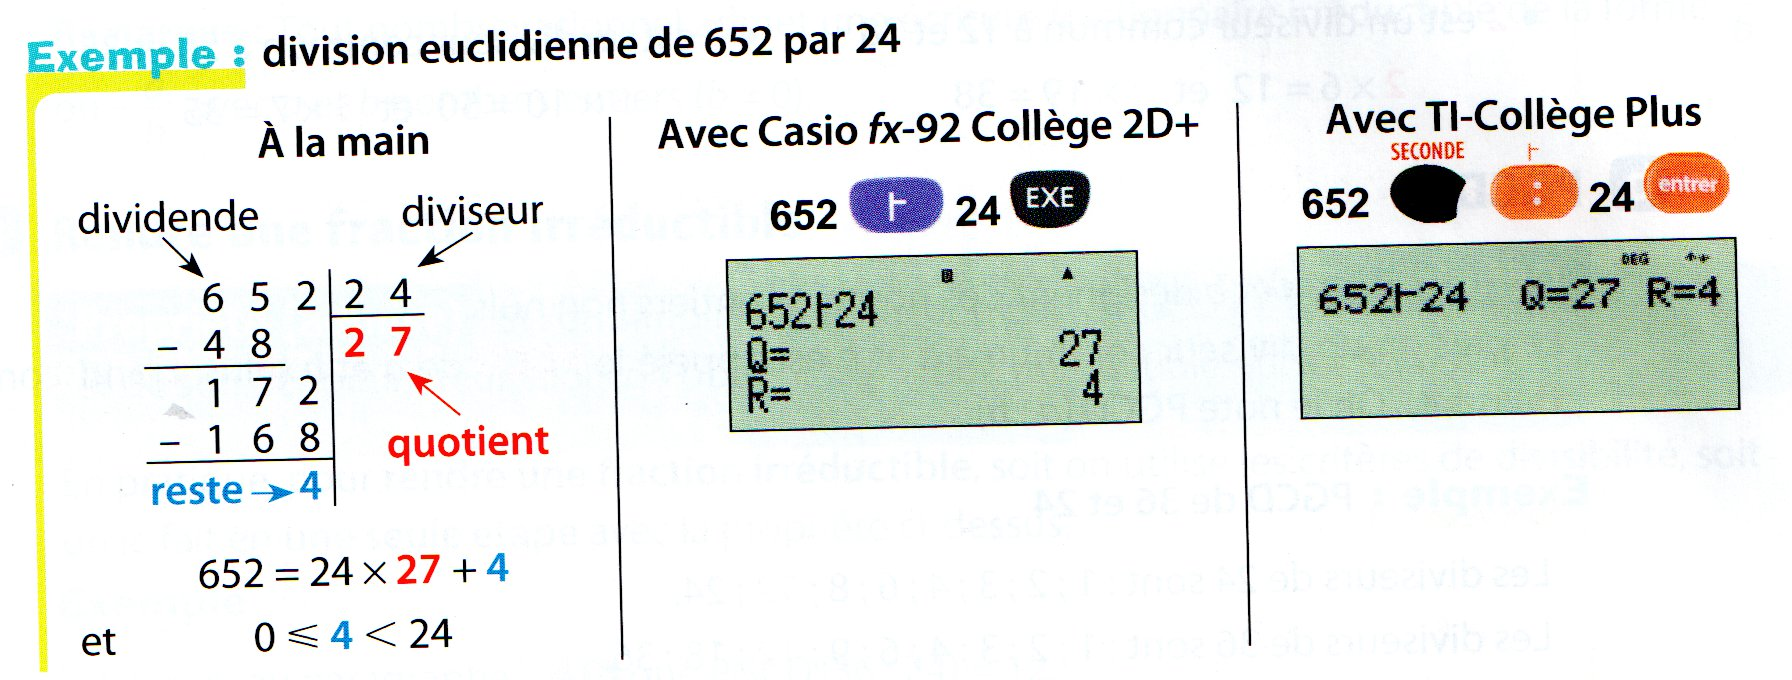
\includegraphics[width=11cm]{images/div.jpg}
\end{center}

\bigskip




\section{Diviser par un nombre entier}

\subsection{Diviseurs et multiples}


\ul{D�finition}: Lorsque le reste de la division euclidienne de $a$ par
$b$ est nul, on dit alors que:

$\bullet$ $a$ est un \textbf{multiple} de $b$

$\bullet$ $a$ est \textbf{divisible} par $b$

$\bullet$ $b$ est un \textbf{diviseur} de $a$.


\bigskip

\ul{Exemple:} $ 36 = 9 \times 4 + 0$. On peut dire:

 36 est un \textbf{multiple} de 9; 
36 est \textbf{divisible} par 9;
9 est un \textbf{diviseur} de 36.



\subsection{Crit�re de divisibilit�}

\ul{Propri�t�}: Un nombre entier est divisible:

\begin{itemize}
  \item [$\bullet$] par 2 lorsque son chiffre des unit�s est 0, 2, 4, 6 ou 8;
  \item [$\bullet$] par 5 lorsque son chiffre des unit�s est 0 ou 5;
  \item [$\bullet$] par 10 lorsque son chiffre des unit�s est 0;
  \item [$\bullet$] par 4 lorsque le nombre form� par les deux derniers
  chiffres (dizaines et unit�s) est divisible par 4;
  \item [$\bullet$] par 3 lorsque la somme de ses chiffres est divisible par 3;
  \item [$\bullet$] par 9 lorsque la somme de ses chiffres est divisible par 9.
\end{itemize}



\bigskip

\ul{Exemple}:

5430 est divisible par 2, 5 et 10 car son chiffre des unit�s est 0.

5430 n'est pas divisible par 4 car 30 n'est pas divisible par 4.

5430 est divisible par 3 mais pas par 9 car 5+4+3+0=12 et 12 est divisible par
3 mais pas par 9.
\end{document}
